\documentclass[14pt]{article}
\usepackage{amsmath,amsthm,amssymb}
\usepackage{mathtext}
\usepackage{amsfonts} 
\usepackage[T1,T2A]{fontenc}
\usepackage[utf8]{inputenc}
\usepackage[english, russian]{babel}
\usepackage[babel=true]{microtype}
\usepackage{caption}
\usepackage{subcaption}
\captionsetup[table]{position=t,justification=raggedleft,slc=off}
\setlength{\abovecaptionskip}{0pt}
\usepackage{geometry}
\usepackage{graphicx}
\usepackage{multirow}
\usepackage{booktabs}
\usepackage{pgfplots}
\usepackage{derivative}
\pgfplotsset{compat=1.18}
\geometry{top=2cm, bottom=2cm, left=2cm, right=1cm}

\title{Отчёт о лабораторной работе №1.3.3. \\ \textbf{Измерение вязкости воздуха по течению в тонких трубках}}
\author{Павел Рудачихин, группа Б04-507}
\date{\today}

\begin{document}
\maketitle

\section*{Аннотация}

\hspace{4mm} В данной работе экспериментально исследуются свойства течения воздуха по тонким трубкам круглого сечения при различных числах Рейнольдса. Изучается переход от ламинарного режима течения к турбулентному, определяется область применимости закона Пуазейля и вычисляется коэффициент динамической вязкости воздуха.

\textbf{Цель работы:} 1) экспериментальное исследование течения газа в тонких трубках; 2) определение границы перехода к турбулентности; 3) измерение коэффициента вязкости воздуха с помощью формулы Пуазейля.

\textbf{Оборудование:} система подачи воздуха (компрессор, подводящие трубки); газовый счётчик барабанного типа ГСБ-400 со счётным устройством; спиртовой микроманометр ММН-2400; набор трубок различного диаметра.

\section*{Теоретические сведения}

\hspace{4mm} Течение вязкой жидкости или газа по прямой трубе круглого сечения вызывается перепадом давления $\Delta P$ на её концах. Силы вязкого трения, препятствующие течению, описываются законом Ньютона:

\begin{equation}
	\tau_{xy} = -\eta \frac{\partial v_x}{\partial y},
\end{equation}
где $\eta$ — коэффициент динамической вязкости среды.

Характер течения определяется безразмерным числом Рейнольдса:
\begin{equation}
	\text{Re} = \frac{\rho \bar{u} R}{\eta},
\end{equation}
где $\rho$ — плотность среды, $\bar{u} = Q/(\pi R^2)$ — средняя скорость потока, $R$ — радиус трубы. При $\text{Re} < \text{Re}_{\text{кр}} \approx 10^3$ течение в трубе является ламинарным, а при превышении критического значения — турбулентным.

В ламинарном режиме для установившегося течения справедлива формула Пуазейля, связывающая объёмный расход $Q$ с перепадом давления $\Delta P$ на участке трубы длиной $l$:

\begin{equation}
	Q = \frac{\pi R^4}{8 \eta l} \Delta P.
\end{equation}

Длина участка установления течения $l_{\text{уст}}$ оценивается по формуле:
\begin{equation}
	l_{\text{уст}} \approx 0,\!2 R \cdot \text{Re}.
\end{equation}

Из кинетической теории газов следует оценка для вязкости идеального газа:
\begin{equation}
	\eta \sim \frac{1}{3} \rho \bar{v} \lambda,
\end{equation}
где $\bar{v}$ — средняя тепловая скорость молекул, $\lambda$ — длина свободного пробега.

Согласно теории размерностей, связь безразмерного перепада давления $\tilde{\psi}$ и числа Рейнольдса имеет универсальный вид:
\begin{equation}
	\tilde{\psi} = C(\text{Re}), \quad \text{где} \quad \tilde{\psi} = \frac{R}{l} \frac{\Delta P}{\rho \bar{u}^2}.
\end{equation}
Для ламинарного течения $C(\text{Re}) \propto 1/\text{Re}$, для турбулентного — $C(\text{Re}) \approx \text{const}$.

\section*{Экспериментальная установка}

\begin{figure}[h!]
	\centering
	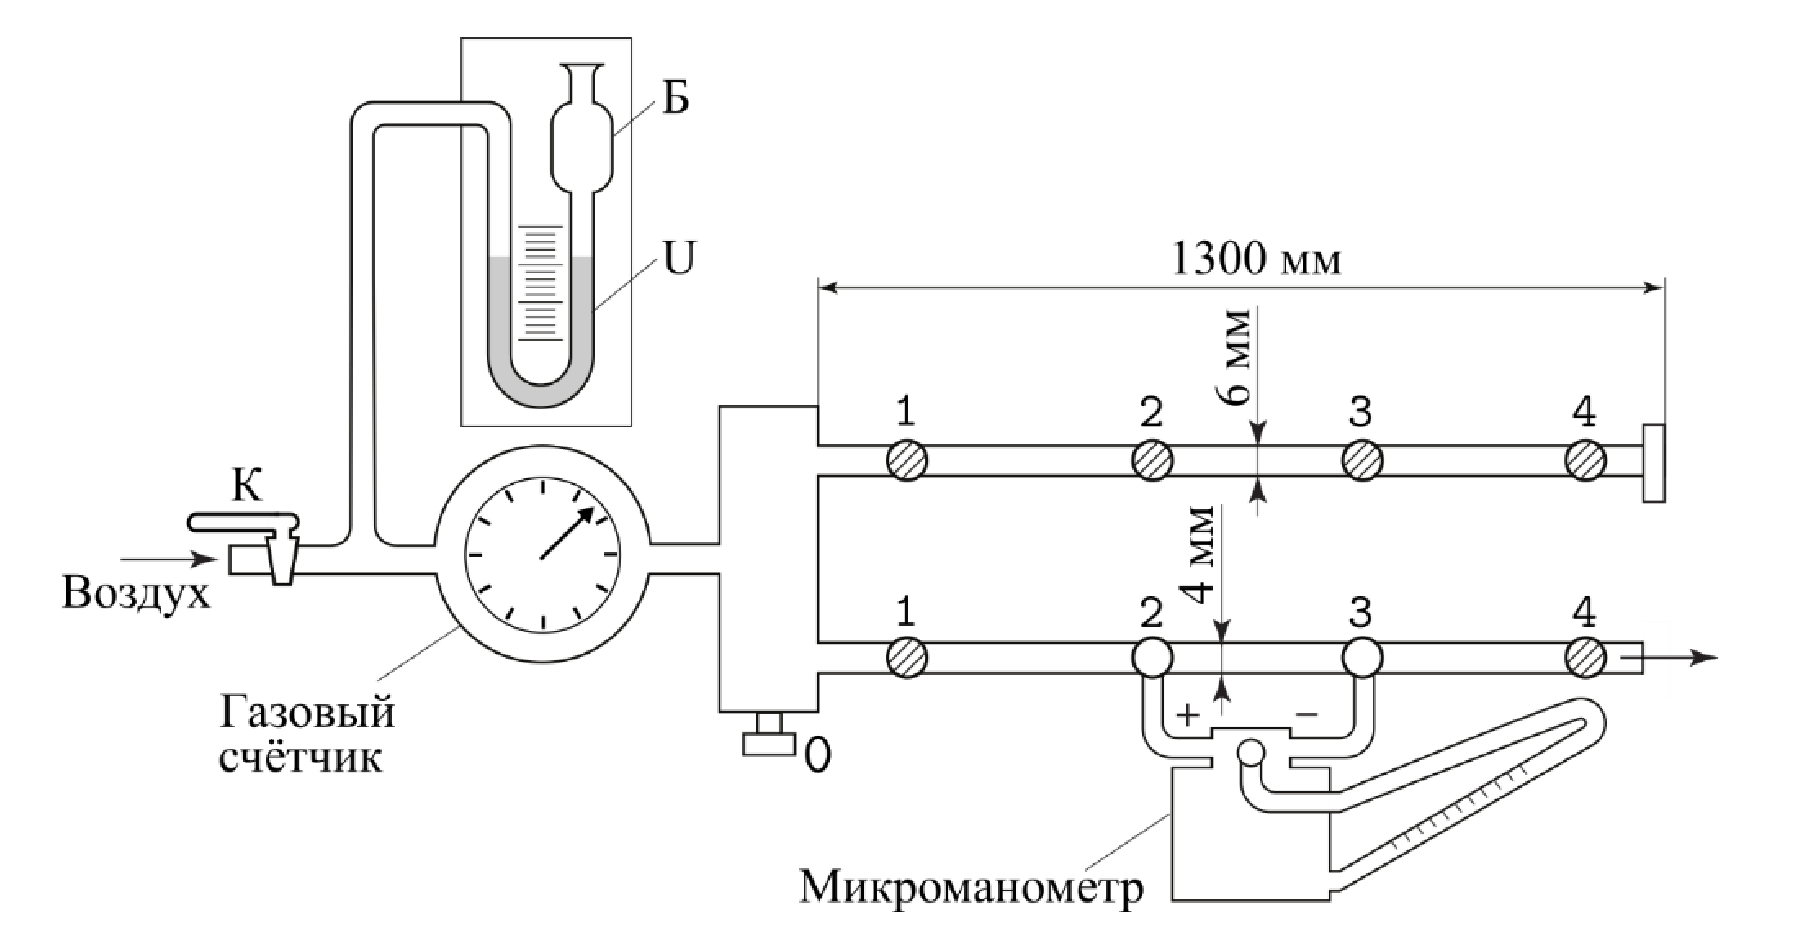
\includegraphics[width=0.7\linewidth]{setup_scheme}
	\caption{Схема установки: 1 — компрессор; 2 — кран К; 3 — U-образный водяной манометр; 4 — газовый счётчик ГСБ-400; 5 — исследуемая трубка с измерительными отверстиями; 6 — микроманометр ММН-2400.}
	\label{fig:setup}
\end{figure}

Поток воздуха от компрессора через кран К и газовый счётчик поступает в одну из исследуемых металлических трубок. Трубки снабжены рядом миллиметровых отверстий для подключения микроманометра. Газовый счётчик барабанного типа ГСБ-400 (класс точности 1,0) измеряет объём прошедшего газа, по которому вычисляется расход $Q = \Delta V / \Delta t$. Микроманометр ММН-2400 с наклонной трубкой (рабочая жидкость — этиловый спирт) измеряет разность давлений между двумя точками трубки. Пределы измерений и цена деления микроманометра зависят от углового коэффициента $K$ (в работе использовалось значение $K = 0,\!2$, цена деления $0,\!20$ мм вод. ст. $\approx 1,\!96$ Па).

\section*{Результаты измерений}

\subsection*{Параметры окружающей среды и установки}

\begin{table}[h!]
	\centering
	\captionbox{Параметры эксперимента}{
	\begin{tabular}{|l|c|}
		\hline
		Температура воздуха $T$, °C & $21,\!9$ \\
		Атмосферное давление $P_A$, кПа & $100,\!13$ \\
		Угловой коэффициент микроманометра $K$ & $0,\!2$ \\
		Поправочный множитель $n$ & $0,\!9953$ \\
		\hline
	\end{tabular}}
\end{table}

\begin{table}[h!]
	\centering
	\captionbox{Геометрические параметры трубок}{
	\begin{tabular}{|c|c|}
		\hline
		№ трубки & $d$, мм \\
		\hline
		1 & $5,\!10 \pm 0,\!05$  \\
		2 & $3,\!00 \pm 0,\!10$  \\
		3 & $3,\!95 \pm 0,\!05$  \\
		\hline
	\end{tabular}}
\end{table}

\subsection*{Зависимость расхода от перепада давления (пункт 7)}

Измерения зависимости $Q(\Delta P)$ проводились для трёх трубок. Расход варьировался краном К от минимального до максимально достижимого. Результаты представлены на рисунке~\ref{fig:QvsDeltaP}. Для каждой трубки на графике выделены ламинарный и турбулентный (переходный) режимы течения.

\begin{figure}[h!]
	\centering
	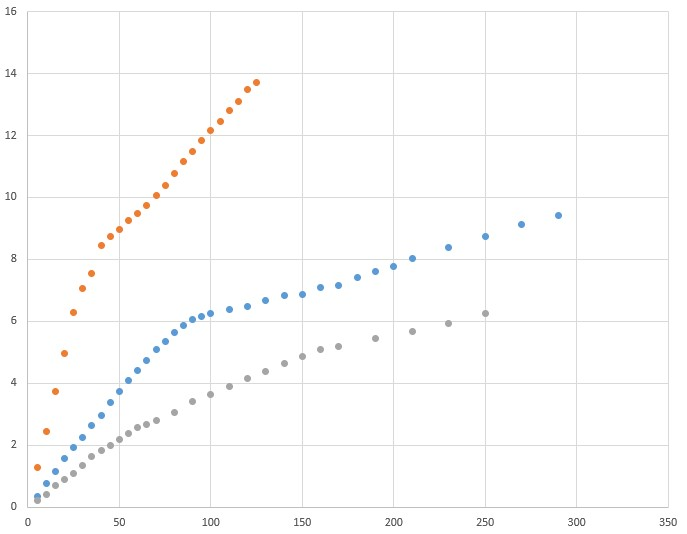
\includegraphics[width=0.7\linewidth]{Screen}
	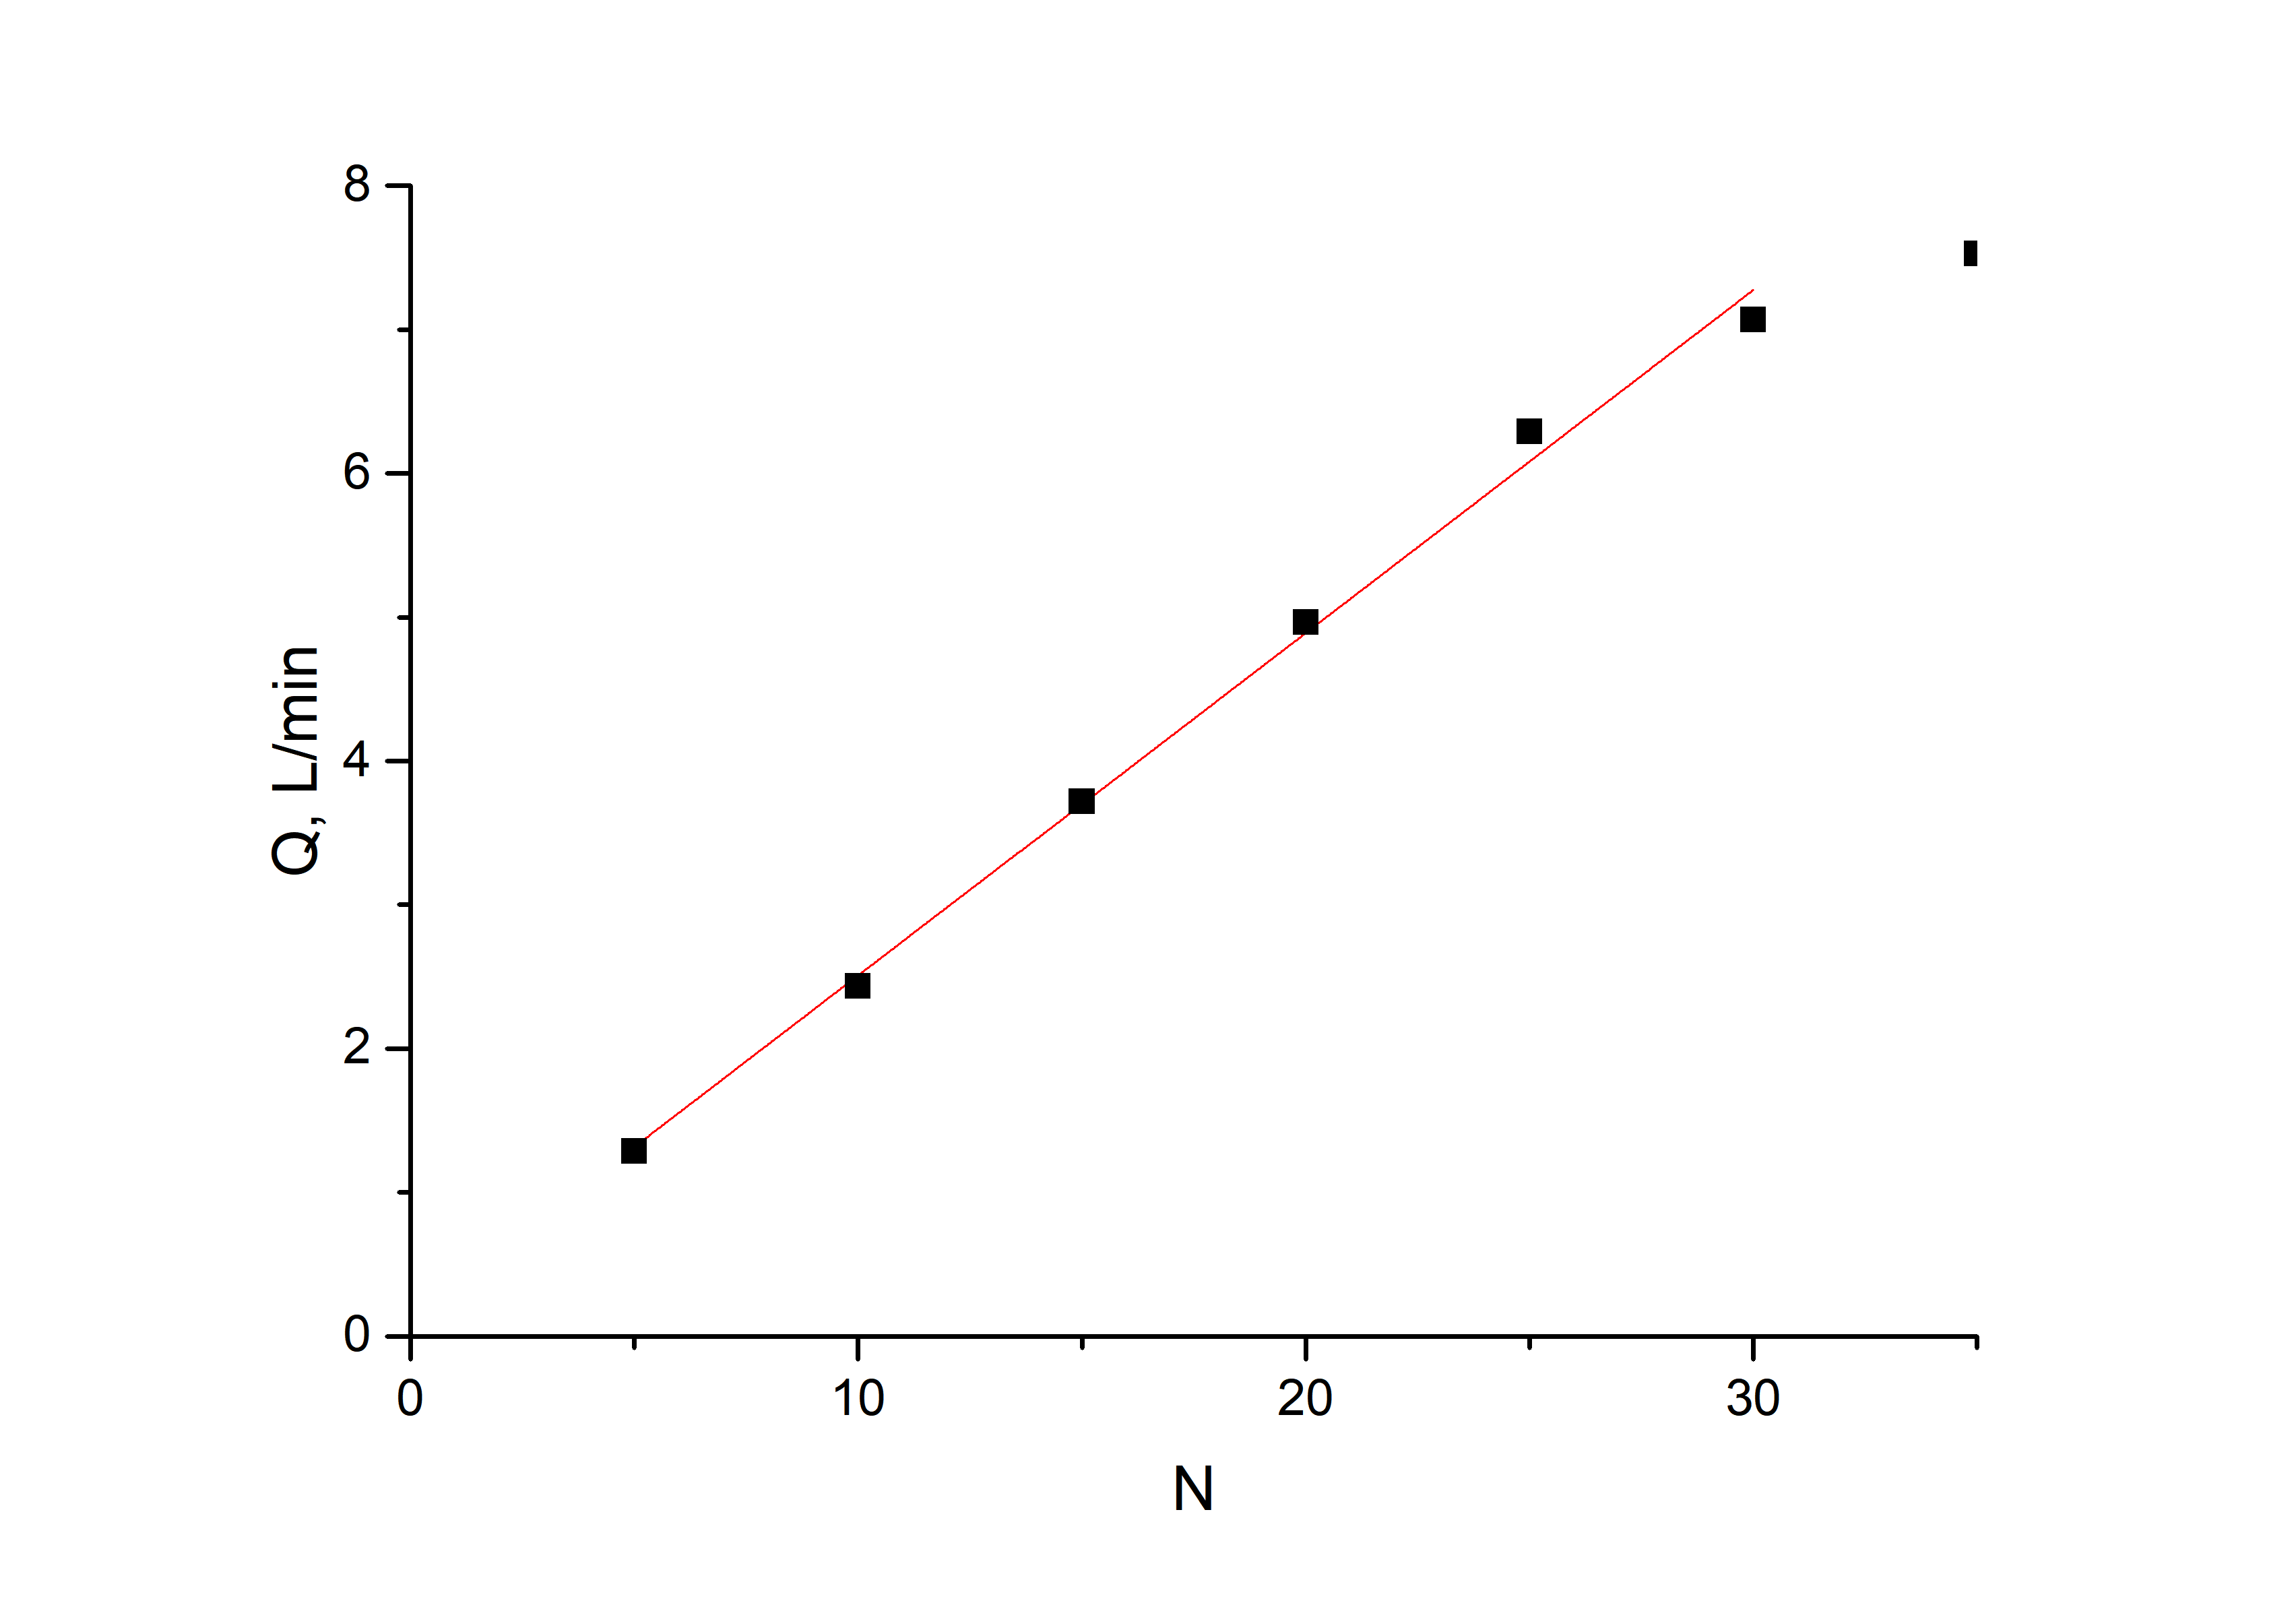
\includegraphics[width=0.3\linewidth]{Graph4}
	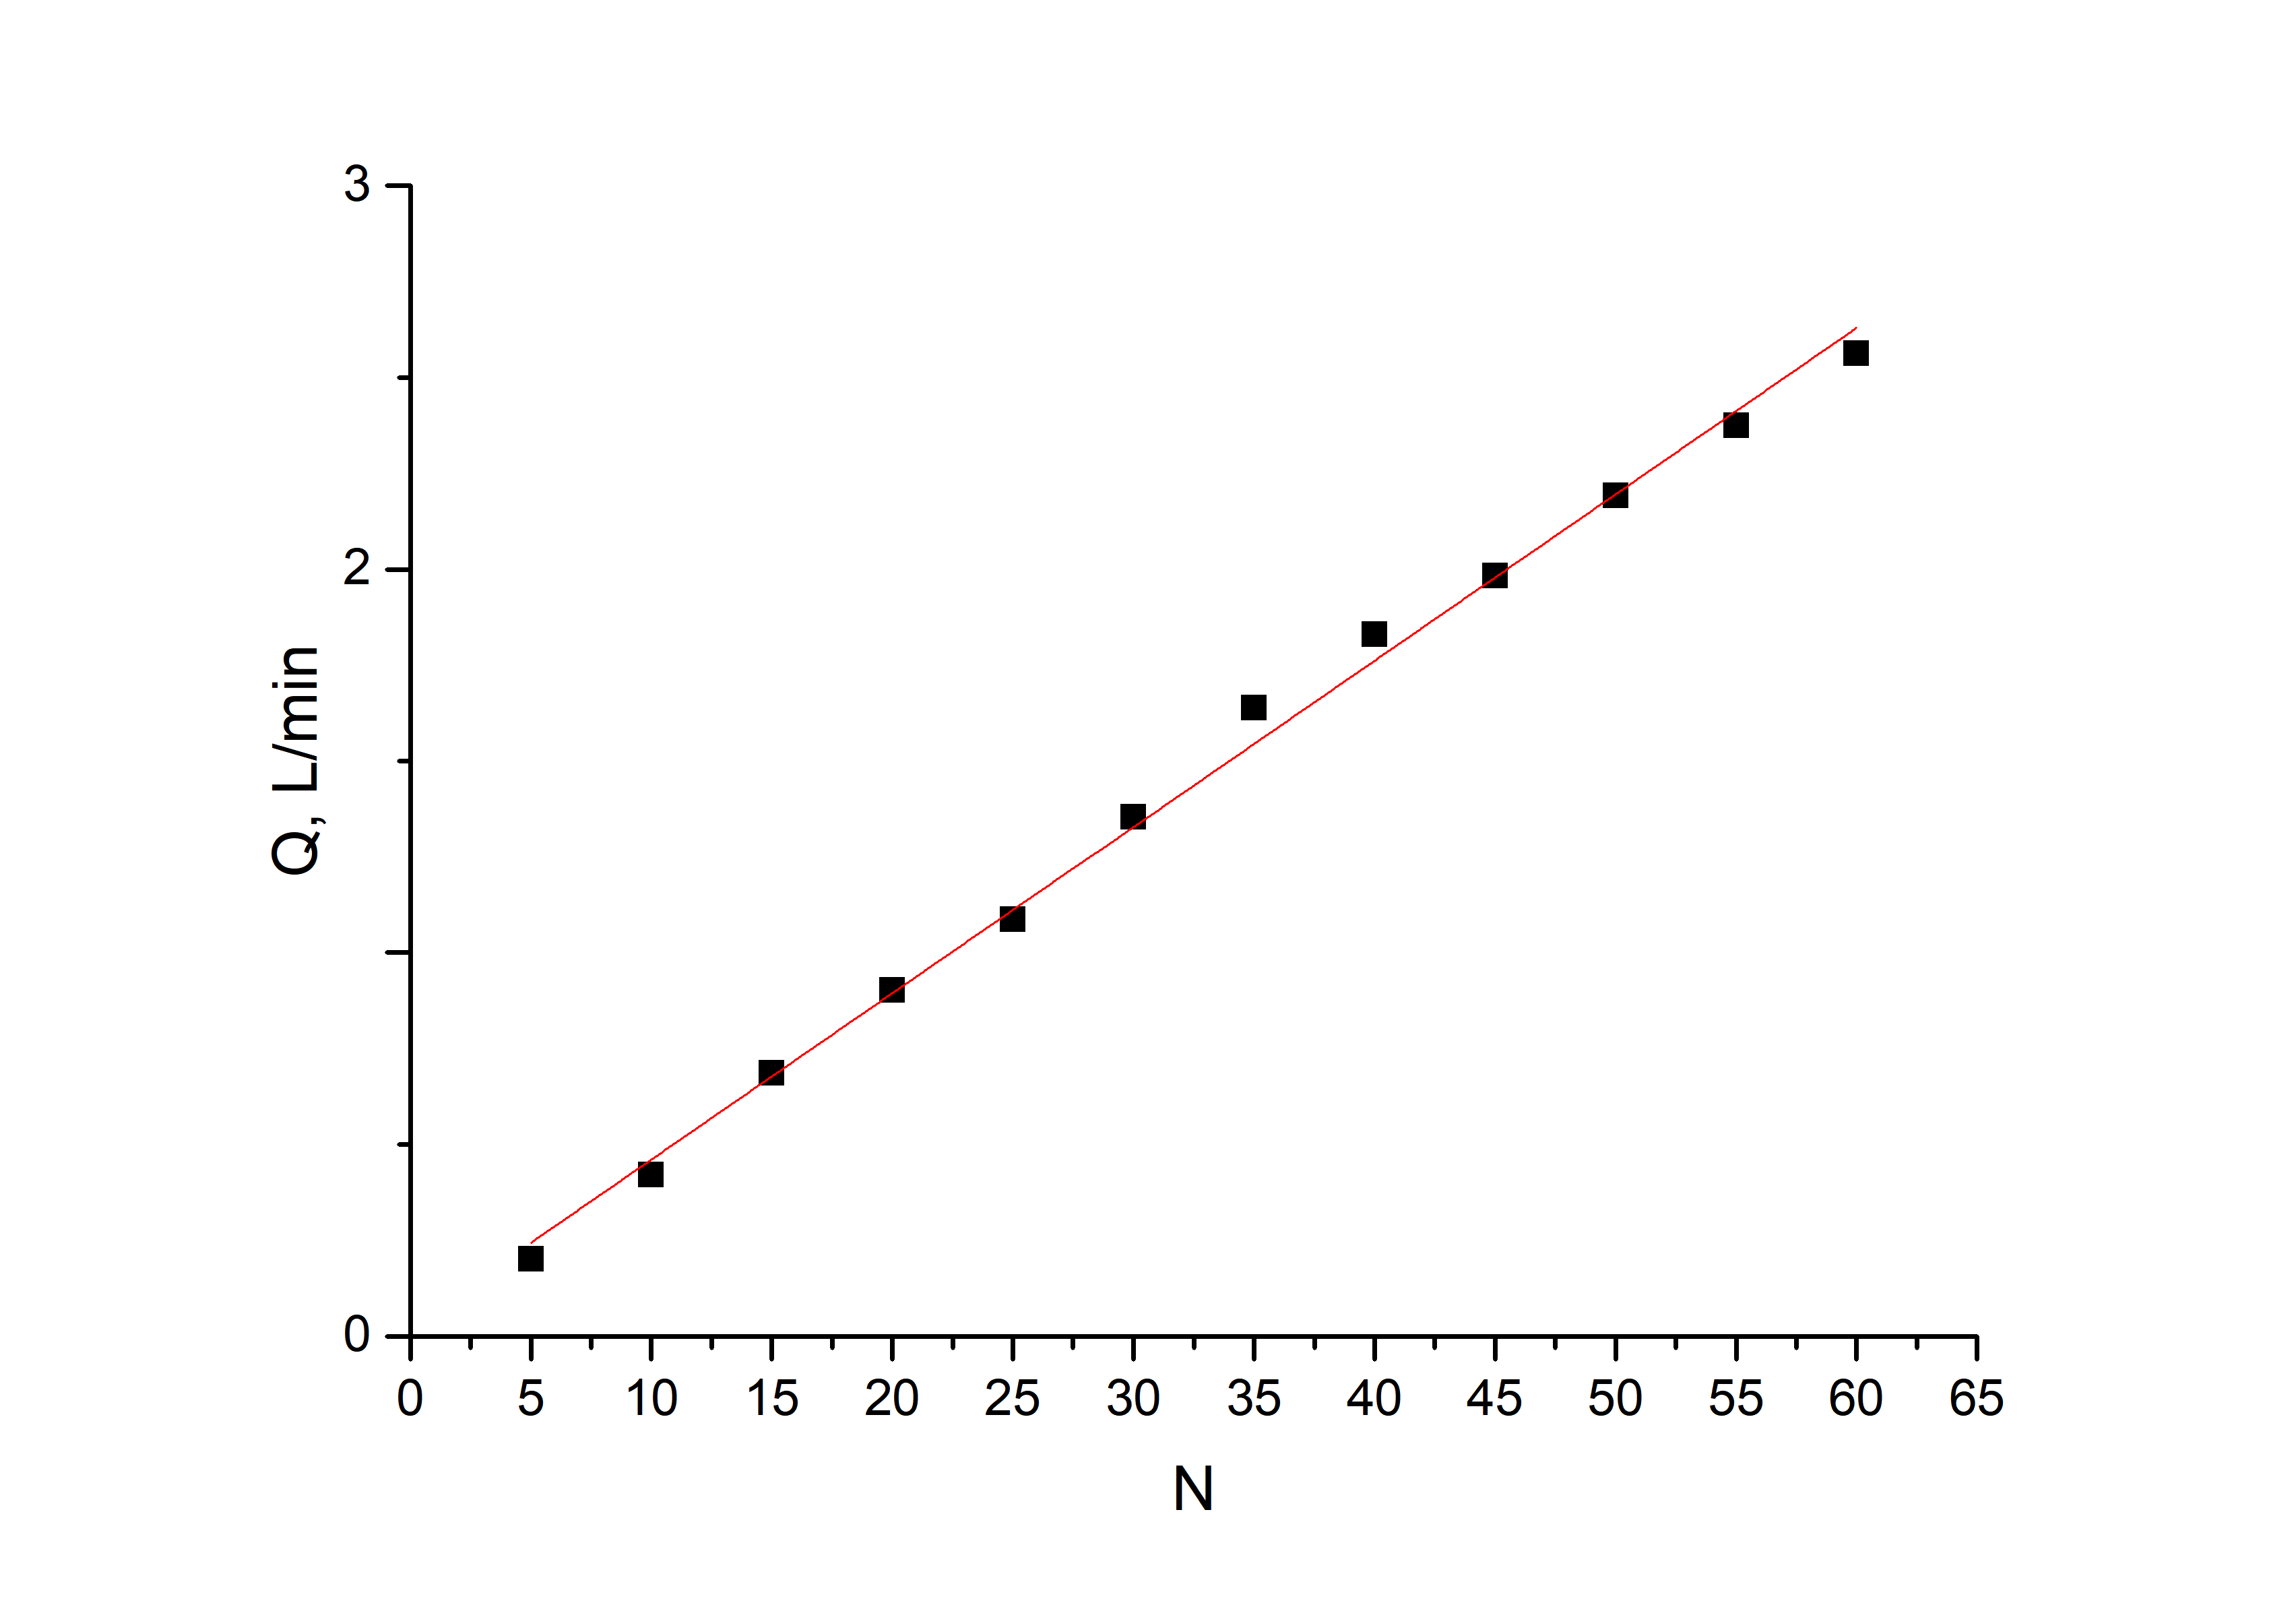
\includegraphics[width=0.3\linewidth]{Graph5}
	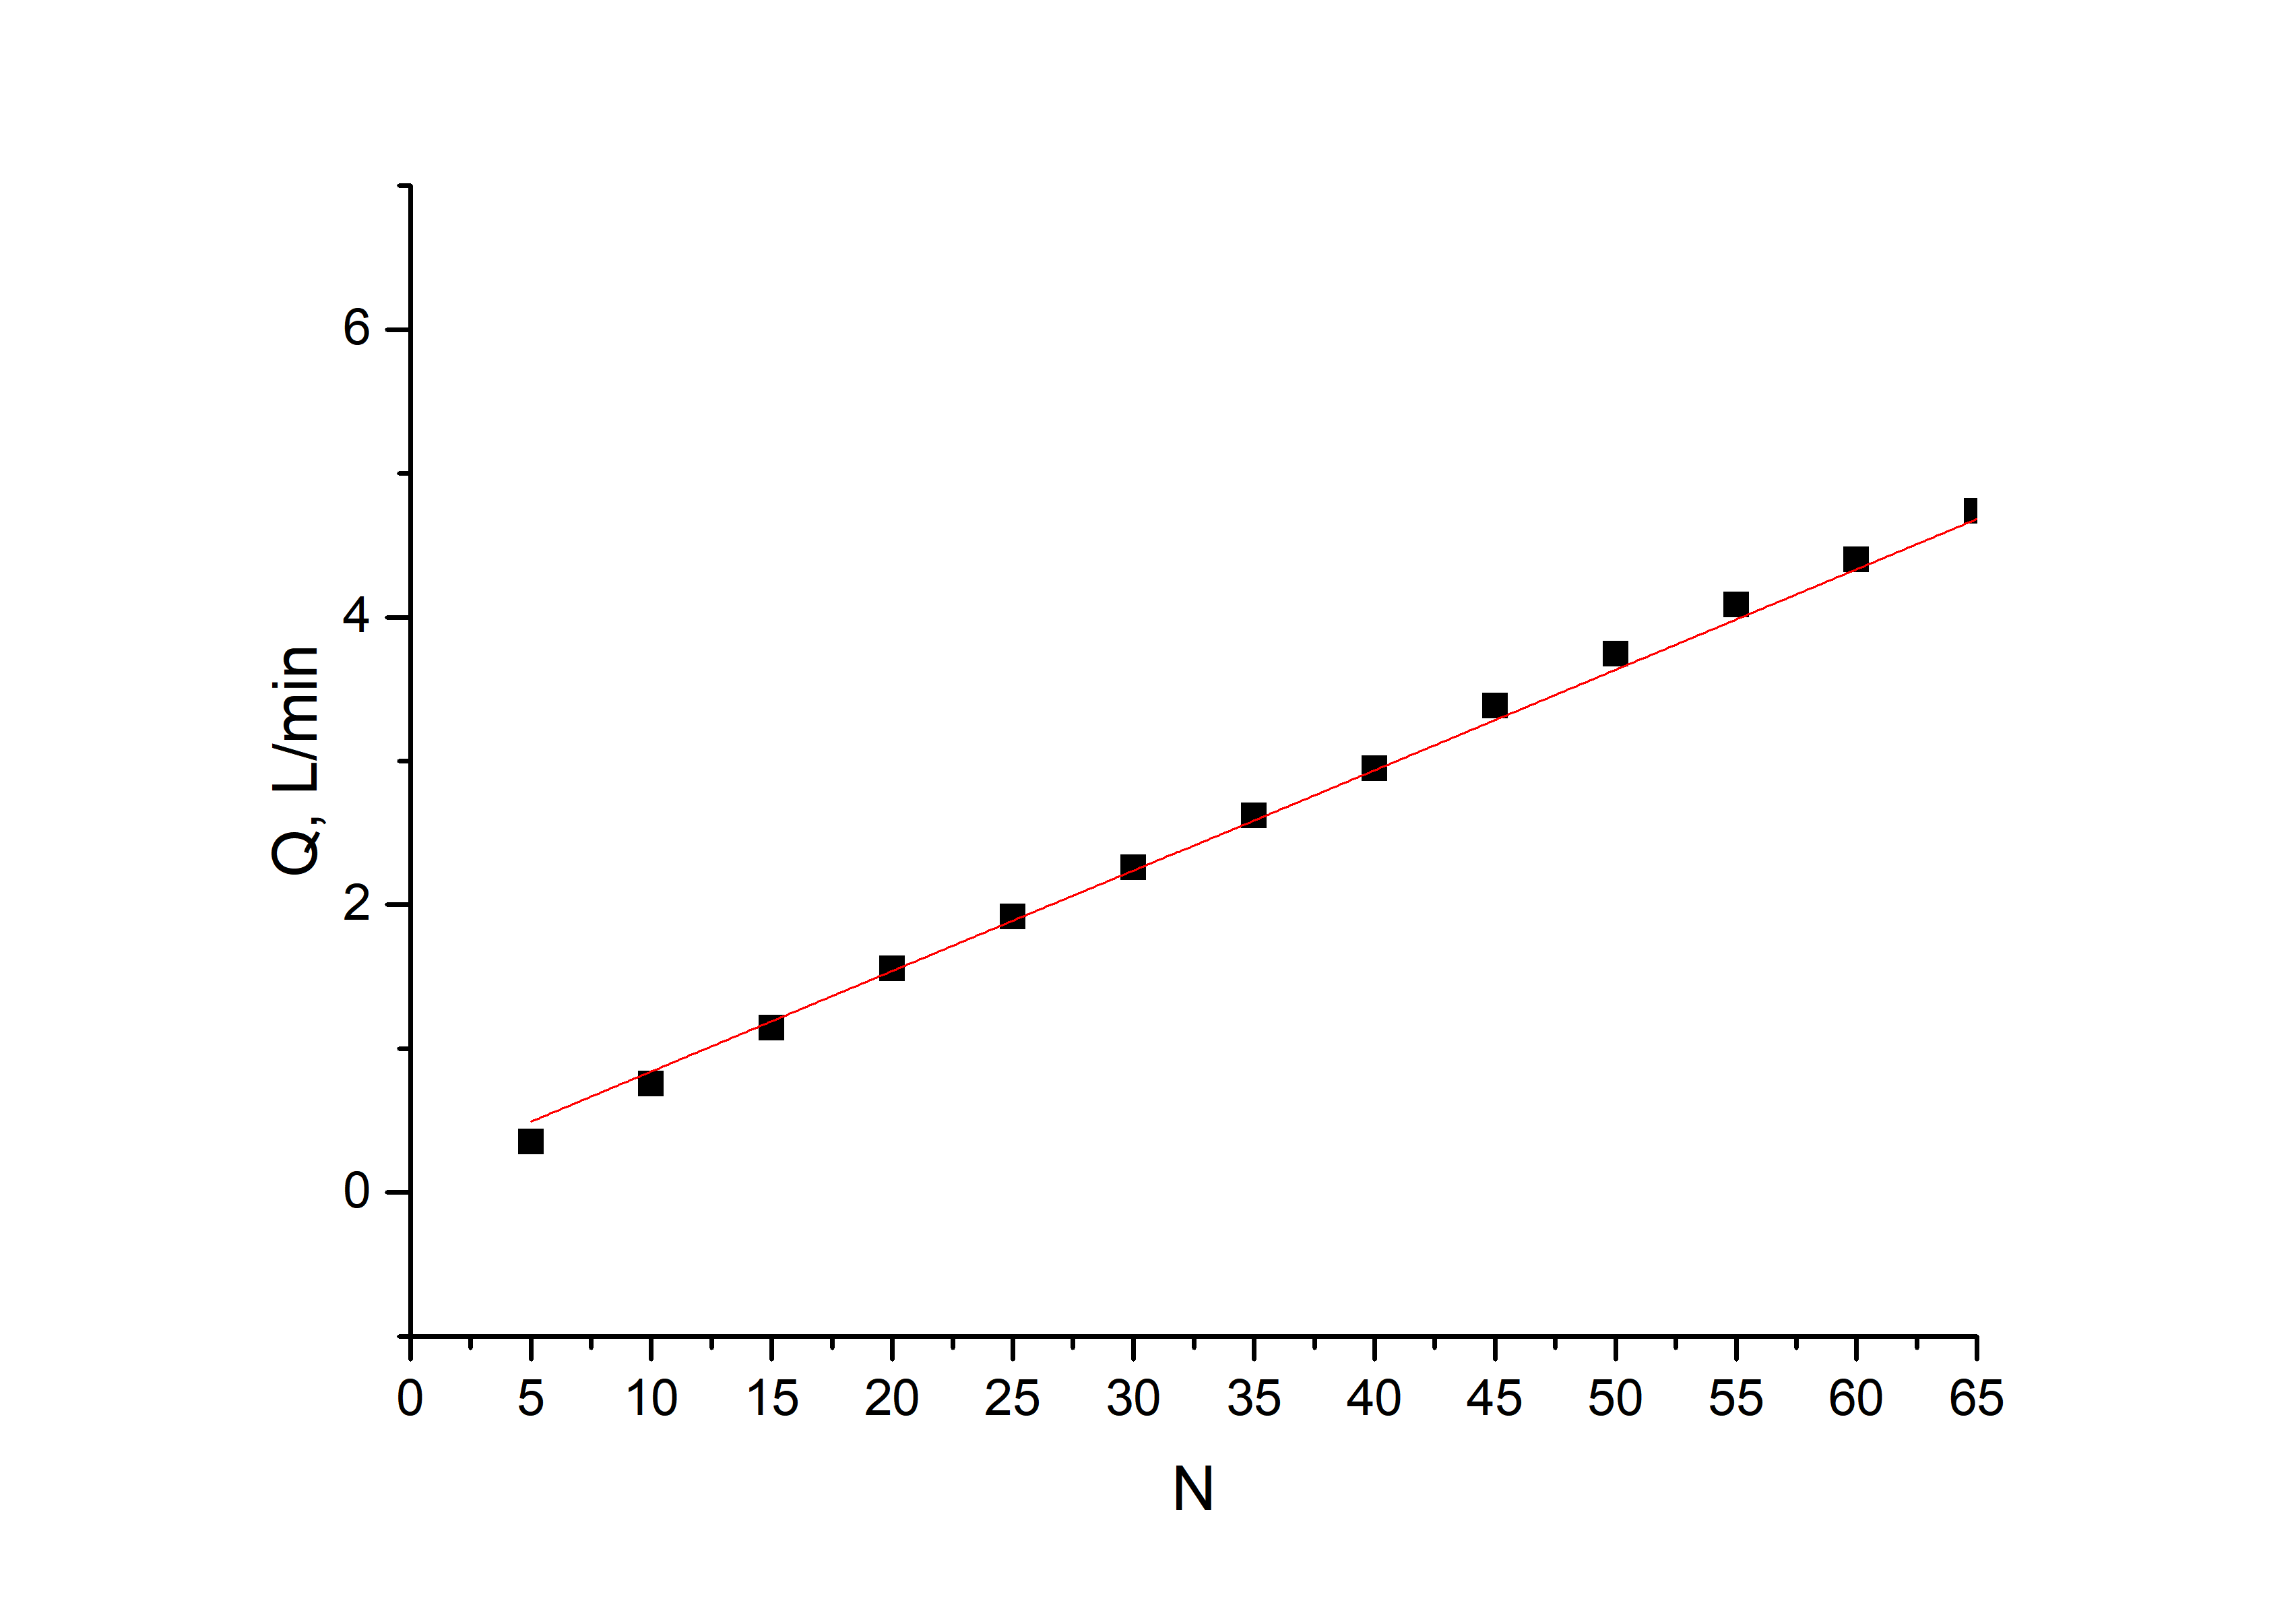
\includegraphics[width=0.3\linewidth]{Graph6}
	\caption{Зависимость расхода $Q$ от перепада давления $\Delta P$ для трёх трубок}
	\label{fig:QvsDeltaP}
\end{figure}

На ламинарных участках зависимость $Q(\Delta P)$ хорошо аппроксимируется прямой линией, что согласуется с формулой Пуазейля. По угловым коэффициентам линейных участков рассчитана вязкость воздуха (таблица~\ref{tab:viscosity}).

\begin{table}[h!]
	\centering
	\captionbox{Результаты расчёта вязкости воздуха}{
	\label{tab:viscosity}
	\begin{tabular}{|c|c|c|c|c|}
		\hline
		№ трубки & $d$, мм & $\eta$, $10^{-5}$ Па$\cdot$с & $\text{Re}_{\text{кр}}$ & $R^2$ ламинарного участка \\
		\hline
		1 & $5,\!10$ & $1,\!64$ & 2345 & $0,\!998$ \\
		2 & $3,\!00$ & $1,\!34$ & 2620 & $0,\!994$ \\
		3 & $3,\!95$ & $2,\!02$ & 1718 & $0,\!999$ \\
		\hline
	\end{tabular}}
\end{table}

Среднее значение вязкости воздуха составило 

\begin{equation*}
	\eta = (1,\!67 \pm 0,\!19) \times 10^{-5} Па \cdot с,
\end{equation*} 
что согласуется с табличным значением $1,\!85 \times 10^{-5}$ Па$\cdot$с при $20^\circ$C.

Критическое число Рейнольдса, определённое по точке перехода от линейной зависимости к нелинейной, по порядку величины соответствует известному из литературы значению $\text{Re}_{\text{кр}} \approx 10^3$.

\subsection*{Распределение давления вдоль трубки (пункт 8)}

Для проверки линейности распределения давления вдоль трубки в ламинарном режиме (формула (4) из описания) были измерены перепады давления на участках различной длины $x$ от начала трубки. Измерения проводились при фиксированном расходе, соответствующем ламинарному режиму ($\Delta P < \Delta P_{\text{кр}}$).

\begin{figure}[h!]
	\centering
	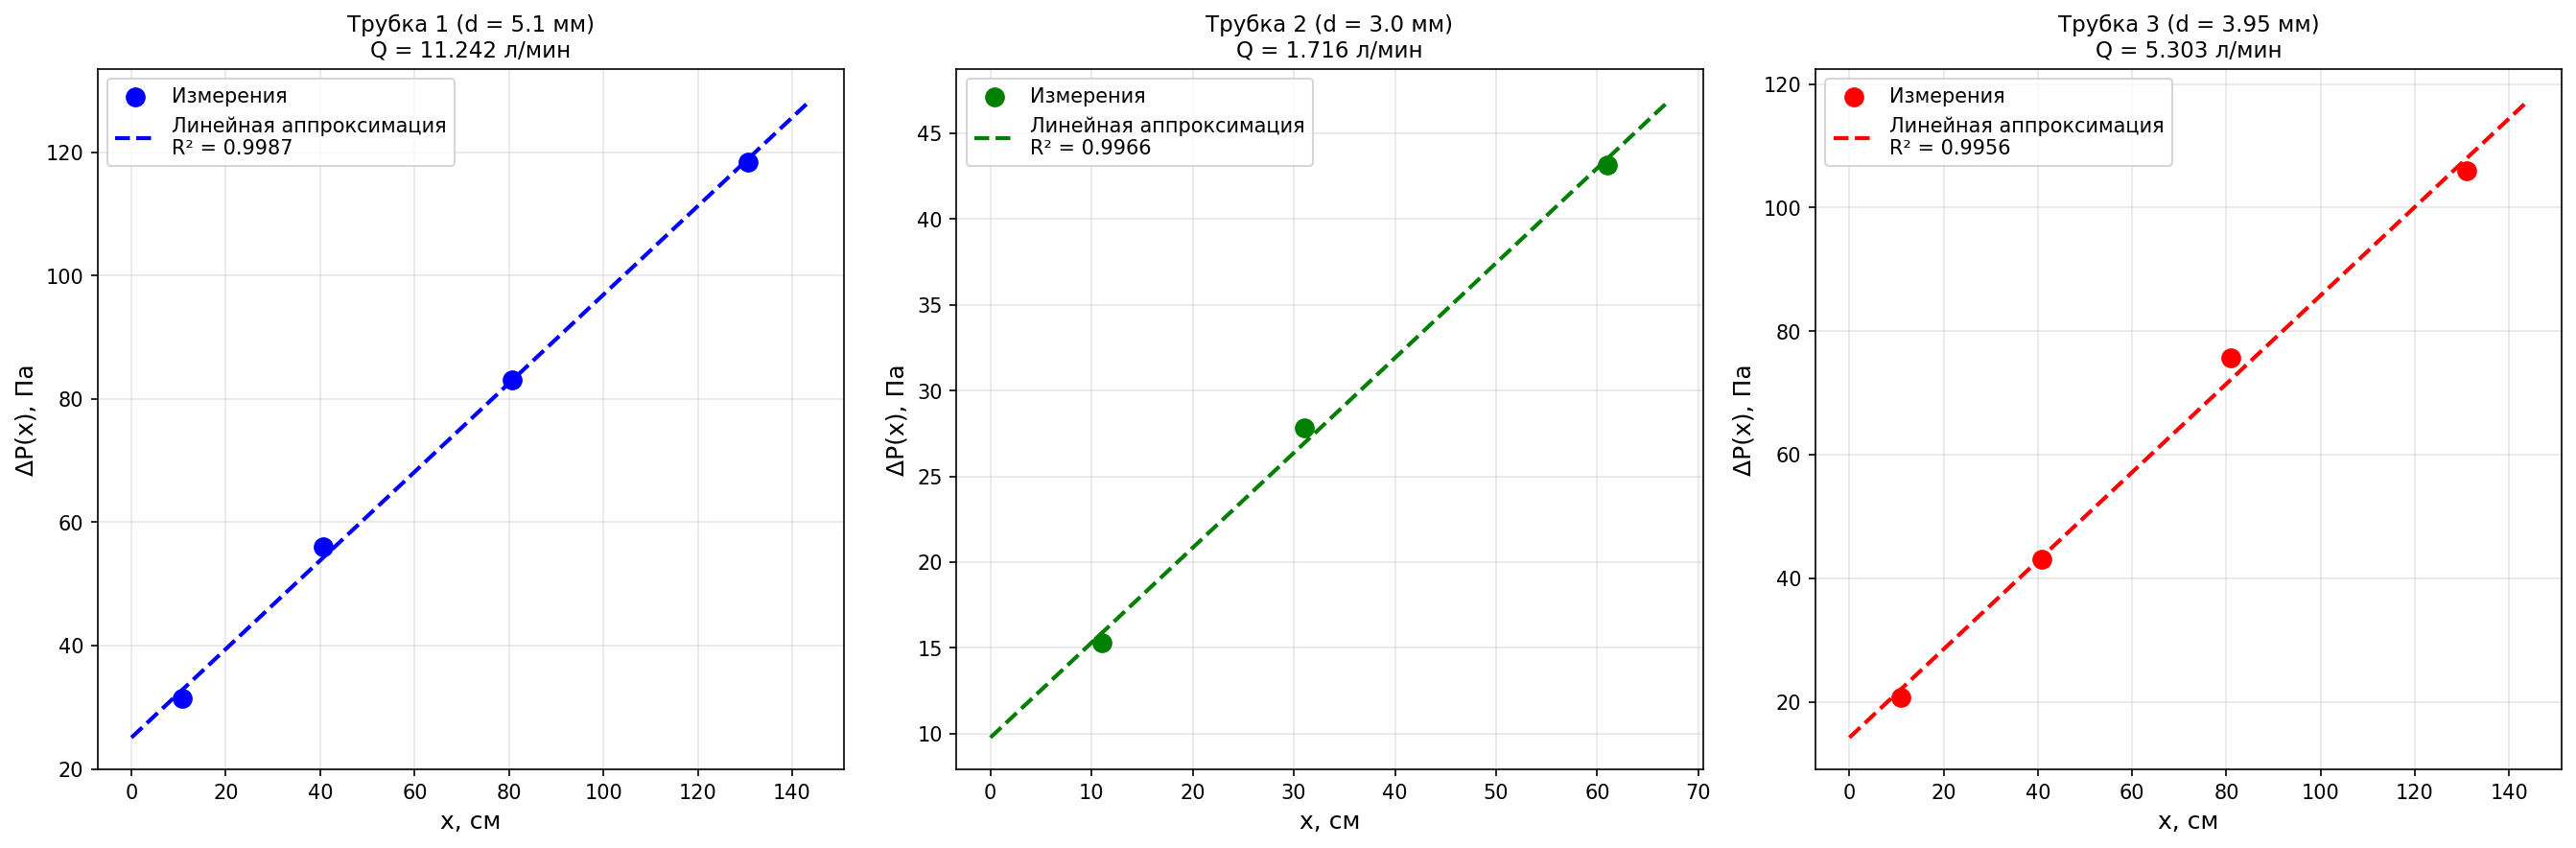
\includegraphics[width=1.0\linewidth]{plots/fig8_pressure_distribution.png}
	\caption{Распределение давления $P(x)$ вдоль трубок в ламинарном режиме.}
	\label{fig:Pdist}
\end{figure}

Как видно из рисунка~\ref{fig:Pdist}, зависимость $P(x)$ близка к линейной для всех трубок. Небольшое отклонение первой точки (наиболее близкой к входу) от линейной экстраполяции может быть связано с участком установления течения. Длина установления, оценённая по формуле (4), составляет $l_{\text{уст}} \approx 0,\!2 R \cdot \text{Re} \sim 10 \div 20$ см для условий эксперимента, что сравнимо с расстоянием до первого измерительного отверстия.

\subsection*{Зависимость расхода от радиуса трубки (пункт 10)}

Для проверки теоретических предсказаний $Q \propto R^4$ (ламинарный режим) и $Q \propto R^{5/2}$ (турбулентный режим) был построен график в двойном логарифмическом масштабе (рисунок~\ref{fig:QvsR}).

\begin{figure}[h!]
	\centering
	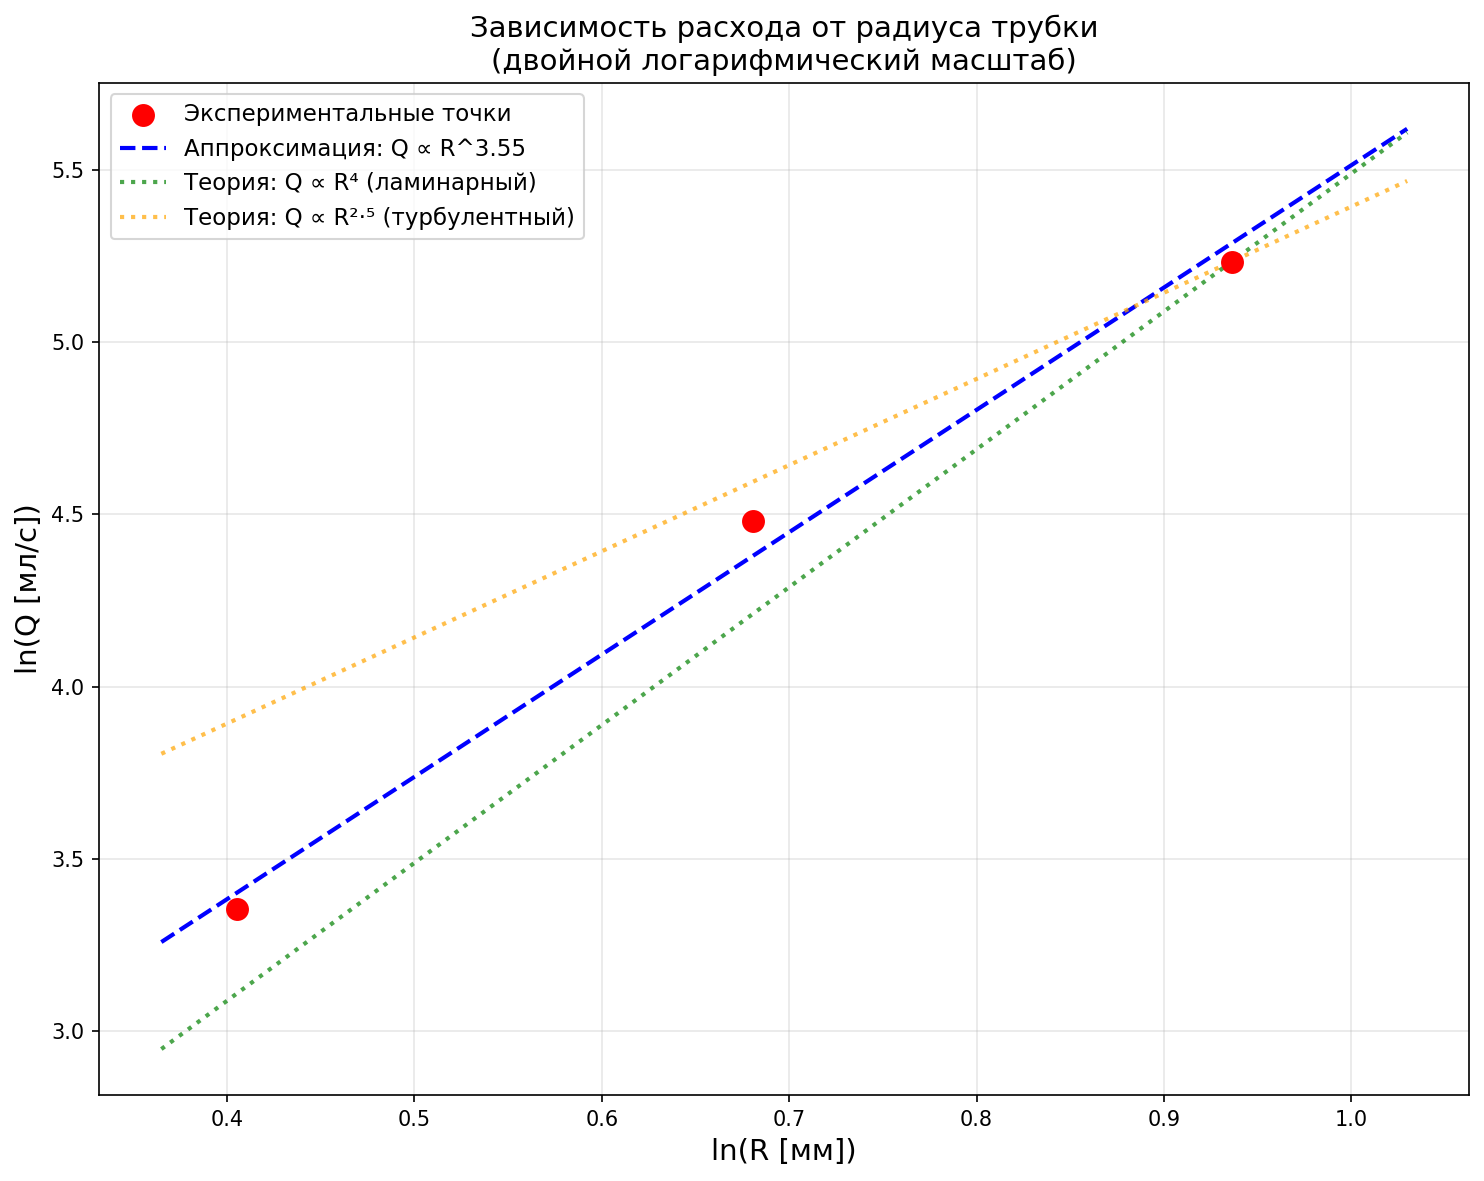
\includegraphics[width=0.8\linewidth]{plots/fig10_Q_vs_R_loglog.png}
	\caption{Зависимость расхода от радиуса трубки в двойном логарифмическом масштабе.}
	\label{fig:QvsR}
\end{figure}

Показатель степени $\beta$ в зависимости $Q \propto R^\beta$, определённый по наклону прямой в логарифмическом масштабе, составил $\beta \approx 3,\!8 \pm 0,\!3$. Это значение ближе к теоретическому $\beta = 4$ для ламинарного режима, что объясняется тем, что измерения в пункте 8 проводились именно в ламинарном режиме.



\section*{Оценка погрешностей}

\subsection*{Инструментальные погрешности}

\begin{itemize}
	\item Погрешность микроманометра ММН-2400: $\sigma_{\Delta P} = 1 \ ед. \approx 1,\!95$ Па при $K=0,\!2$.
	\item Погрешность газового счётчика ГСБ-400 (класс точности 1,0, цена деления $0,\!003$ л): $\sigma_V = 0,\!003$ л.
	\item Погрешность измерения диаметра трубок: $\sigma_d = 0,\!05 \div 0,\!10$ мм.
\end{itemize}

\subsection*{Погрешность измерения вязкости}

Относительная погрешность определения вязкости по формуле Пуазейля:
\begin{equation}
	\varepsilon_\eta = \sqrt{\left(4 \frac{\sigma_R}{R}\right)^2 + \left(\frac{\sigma_l}{l}\right)^2 + \varepsilon_Q^2 + \varepsilon_{\Delta P}^2}.
\end{equation}

Основной вклад в погрешность вносит неточность измерения радиуса трубки (умноженная на коэффициент 4). Для трубки 2 ($d = 3,\!00 \pm 0,\!10$ мм) относительная погрешность $\varepsilon_\eta$ достигает $15\%$, для трубок 1 и 3 — около $5\%$.

Случайная погрешность, оценённая по разбросу значений $\eta$ для разных трубок, составила $\sigma_\eta \approx 0,\!09 \times 10^{-5}$ Па$\cdot$с, что соответствует относительной погрешности около $5\%$.

\subsection*{Погрешность числа Рейнольдса}

\begin{equation}
	\varepsilon_{\text{Re}} = \sqrt{\varepsilon_\rho^2 + \varepsilon_u^2 + \varepsilon_R^2 + \varepsilon_\eta^2} \approx 20\%.
\end{equation}

\section*{Заключение}

\hspace{4mm} В ходе выполнения работы были достигнуты поставленные цели:

\begin{enumerate}
	\item Экспериментально исследован характер течения воздуха в тонких трубках круглого сечения при различных числах Рейнольдса. Обнаружен переход от ламинарного режима к турбулентному при $\text{Re}_{\text{кр}} \approx 2 \times 10^3$, что согласуется с известным из литературы значением.
	\item Подтверждена линейная зависимость расхода от перепада давления $Q \propto \Delta P$ на ламинарном участке в соответствии с формулой Пуазейля.
	\item Определён коэффициент динамической вязкости воздуха: $\eta = (1,\!67 \pm 0,\!19) \times 10^{-5}$ Па$\cdot$с, что совпадает с табличным значением при комнатной температуре.
	\item Проверено распределение давления вдоль трубки $P(x)$ — зависимость близка к линейной, что характерно для установившегося ламинарного течения.
\end{enumerate}

Основным источником погрешностей является неточность измерения диаметра тонких трубок, что особенно существенно для трубки наименьшего диаметра (3,\!00 мм).

\end{document}